%% LaTeX Boilerplate (http://github.com/gbluma/latex-boilerplate/)
%% https://www.overleaf.com/learn/latex/Learn_LaTeX_in_30_minutes#Writing_your_first_piece_of_LaTeX

\documentclass[11pt,a4paper]{article}
\usepackage[a4paper, top=1cm, bottom=2cm, left=2.5cm, right=2.5cm]{geometry}
\usepackage{indentfirst}
\usepackage[indent=0em]{parskip}
\usepackage[utf8]{inputenc}
\usepackage[T1]{fontenc}
\usepackage{helvet} %lmodern
\usepackage{graphicx}
\usepackage[hidelinks]{hyperref}
\renewcommand{\familydefault}{\sfdefault}

\graphicspath{ {./images/} }

\title{TP INF727 \textbf{Implémentation de Hadoop MapReduce "from scratch" en Python}}
\author{Pierre Dal Bianco}
\date{}

\begin{document}

\maketitle
\hrulefill

L'ensemble du code pour ce projet est disponible sur GitHub à l'adresse suivante : \url{https://github.com/pierre-db/INF727_Distributed-Project}.

\section*{Introduction}
Pour ce projet nous allons coder un programme de comptage de mots en MapReduce. Nous allons essayer de comprendre les limitations de la méthode telle qu'elle a été décrite par Google en 2004 ainsi que les optimisations que nous pourrons effectuer dans notre cas spécifique. Il sera de plus intéressant de comparer les temps d'execution par rapport à un comptage de mots séquenciel ainsi que d'observer l'évolution du temps d'execution d'une tâche en fonction du nombre de workers, puisque nous disposons grace aux machines de l'école de machines aux caractéristiques techniques plus ou moins équivalentes entre elles. Il sera notamment intéressant de comparer nos résultats à la loi d'Amdahl.

L'ensemble du code (qui est disponible sur \href{https://github.com/pierre-db/INF727_Distributed-Project}{GitHub}) a été executé sur les machines de l'école, y compris le code pour le master afin d'utiliser un parc de machines cohérent et de réduire les temps de communications réseau entre machines. La liste exhaustive des machines utilisées est disponible dans le fichier \texttt{machines.txt}, la machine tp-4b01-00 qui n'est pas dans cette liste a été utilisée comme master, afin d'éviter d'utiliser une même machine à la fois comme worker et comme master.

Dans la suite de ce document nous allons revenir sur les difficultés et les optimisations que nous pouvons faire pour chacune des étapes de base d'une opération MapReduce : Split $\rightarrow$ Map $\rightarrow$ Shuffle $\rightarrow$ Reduce, ainsi que l'étape de récupération des résultats par le master ici désignée par le terme Fetch.

\section{Split}
La difficulté pricinpale sur cette étape a été de découper et répartir le ficher sur lequel on souhaite faite le word count entre les workers. Une première approche pourrait être de charger tout le fichier en RAM sous forme d'un \texttt{string} avec \texttt{file.read()}, d'en déduire le nombre de caractères avec la fonction \texttt{len()} et de travailler sur les indices du \texttt{string} pour écrire chaque morceau dans un fichier séparé. Pour des fichiers de grosse taille, notamment sir la taille du fichier excède l'espace RAM disponible, cette approche peut être problématique.

L'approche privilégiée a été de lire la taille du fichier en octets avec la fonction \texttt{os.path.getsize (filename)}. On peut ensuite découper le fichier en n (n = nombre de workers) blocs de taille = taille du fichier / nombre de workers. On peut alors lire le fichier par blocs de taille constante et écrire ces blocs dans des fichiers séparés. Une petite astuce pour éviter de découper un mot est de lire le dernier caractère de chaque bloc et d'ajouter au bloc en cours tous les caractères qui suivent jusqu'à ce qu'on tombe sur un espace ou une nouvelle ligne. Une limite de cette approche est que la taille du fichier en octets n'est pas nécessairement égale au nombre de caractères dans le fichier. Les caractères encodés en UTF-8 font au moins un octet mais peuvent aussi faire plus dans le cas d'un caractère non latin. Cette méthode a donc tendance à surestimer la taille de chaque bloc. On peut donc se retrouver avec le dernier fichier du split vide. On considèrera cependant ici que le gain de temps et d'utilisation de RAM sont suffisants pour justifier ce compromis.

\section{Map}
Cette étape est assez directe, il s'agit d'envoyer les splits vers les workers puis de découper chaque ligne du split au niveau des caractères blancs (*white space caracters*). On écrit ensuite chaque mot dans un fichier.

Le plus long à cette étape est l'envoi des splits. La partie \textit{Accélerer les transferts scp} décrit comment les temps de transferts scp ont été (légèrement) améliorés.

\section{Shuffle}
\subsection*{Accélerer le shuffle}
Pour le shuffle l'implémentation initiale créait un fichier par hash (i.e. par mot) et par worker. Cela génèrait une quantité importante de petits fichiers qui doivent ensuite être écrits sur disque, transférés entre les workers et lus. Cela posait problème pour deux raisons : les transferts entre machines, et les temps d'écriture sur disque.

Lors des transferts entre machines, le programme initial générait la liste de fichiers à envoyer à chaque machine et passait la liste de fichiers en argument à la commande scp. Cela évitait de faire une commande scp par fichier, mais génerait un nombre trop important d'arguments. Avec le fichier \texttt{sante\_publique.txt} de 18.3 MB et 3 workers, le programme générait un peu plus de 9000 arguments (1 argument = 1 fichier) à chaque commande scp. Cela produisait une erreur du fait que le nombre maximum d'arguments était dépassé et la commande scp échouait. Une première amélioration a consisté à mettre tous les fichiers destinés à une machine dans un même répertoire, puis de simplement passer le nom du répertoire en argument à scp. 

Les temps de lectures et d'écritures séquenciels étant assez élevés, l'approche qui consiste à génerer un fichier par mot n'est pas optimale et génère beaucoup de latence. Sur le fichier \texttt{sante\_publique.txt} de 18.3 MB avec 3 workers, le shuffle prennait 35s.


\includegraphics[width=5cm]{screenshot_shuffle1.png}

Le fichier \texttt{CC-MAIN-20170322212949-00140-ip-10-233-31-227.ec2.internal.warc.wet} (398.8 MB) ne parviennait pas à terme du shuffle (problèmes de timeout et du nombre trop important de requêtes simultanée par worker).

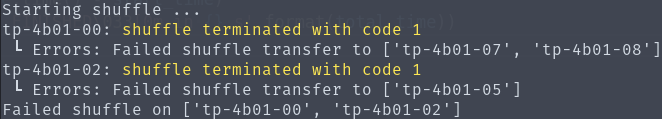
\includegraphics[width=10cm]{screenshot_shuffle2.png}

La solution a été de créer un fichier par machine qui contient pour chaque machine les mots qui lui sont attribués par la fonction de hashage. Dans un premier temps, les mots sont écrits à la suite d'un fichier au fur et à mesure qu'ils sont traités. Après cette optimisation, le shuffle sur le fichier de 18.3 MB prend 23 secondes avec 3 workers.


\includegraphics[width=5cm]{screenshot_shuffle3.png}

Sur le fichier de 398.8 MB, le shuffle parvient alors à terme et prend 7 min 10s avec 3 workers.


\includegraphics[width=5cm]{screenshot_shuffle4.png}

Enfin, pour gagner encore plus en performance, la dernière amélioration consiste à écrire les shuffles dans un dictionnaire (l'équivalent Python d'une table de hashage) en mémoire RAM et d'écrire les fichiers issus du shuffle en une seule opération, une fois tous les résulats aggrégés en RAM. Le gain de performance est assez conséquent, mais peut poser problème dans le cas où les shuffles ne tiennent pas en RAM. Après cette optimisation, le shuffle sur le fichier de 18.3 MB prend 2 seconde avec 3 workers.


\includegraphics[width=5cm]{screenshot_shuffle5.png}

Sur le fichier de 398.8 MB, le shuffle ne prend plus que 30s avec 3 workers.


\includegraphics[width=5cm]{screenshot_shuffle6.png}


\section{Reduce}
\subsection*{Accélerer la récupération et l'aggrégation des résultats}
Le code initial créait un fichier de la forme \texttt{<hash>.txt} par mot au moment du reduce. Cela  impliquait la création d'un total d'environ 56 000 fichiers (chacun correspondant à un mot unique) qui étaient ensuite récupérés par scp vers le master. Le master devait ensuite ouvrir chacun de ces fichiers pour récupérer les mots et leur compte, avant de concaténer tous les mots en mémoire (RAM), de les trier par order d'occurences puis les afficher. Sur le fichier \texttt{sante\_publique.txt} (18.3 MB), l'étape de récupération et de concaténation de ces fichiers prenait 1 min 42s. À la vue de ce résultat cette configuration n'a pas été testée sur le fichier de 398.8 MB.

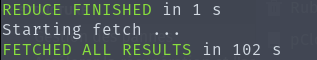
\includegraphics[width=5cm]{screenshot_reduce1.png}

L'amélioration consiste ici à écrire tous les mots et leur compte respectif issus du reduce dans un seul fichier par worker. Dans un premier temps les écritures sur disque sont faites ligne par ligne. Le master récupère ensuite ces fichiers via scp, et récupère ensuite toutes les lignes de chaque fichier. On passe d'un fichier par mot à un fichier par worker. Sur le fichier \texttt{sante\_publique.txt} avec 3 workers, l'étape de récupération et de concaténation deviens alors quasi instantanée (< 1 sec).


\includegraphics[width=5cm]{screenshot_reduce2.png}

Sur le fichier de 398.8 MB avec 3 workers cette étape (reduce + fetch) prend 32 secondes.


\includegraphics[width=5cm]{screenshot_reduce3.png}

La dernière amélioration sur cette étape, comme pour le shuffle consiste à écrire le fichier reduce en une seule fois en écrivant les résutats intermédiaires en RAM. Avec cette amélioration, sur le fichier de 398.8 MB avec 3 workers le réduce prend 8 secondes.

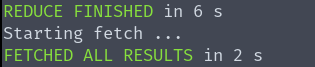
\includegraphics[width=5cm]{screenshot_reduce4.png}

\section{Autres améliorations}
\subsection*{Accélerer les transferts scp}
La majorité des délais sont liés aux transferts de fichiers entre les workers entre eux (shuffle) et avec le master (split, recupération des reduces). Une amélioration consiste simplement à passer l'option \texttt{-C} à scp pour compresser automatiquement les fichiers à transférer. Avant cette optimisation, sur le fichier de 398.8 MB avec 5 workers, les temps des différentes étapes étaient les suivantes : split : 7s, map : 19s, shuffle : 22s, reduce : 5s, recupération des réduce : 3s.

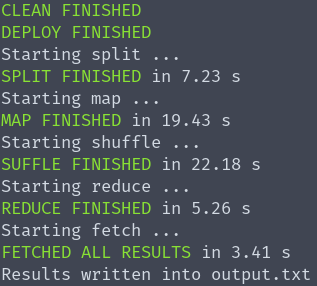
\includegraphics[width=5cm]{screenshot8.png}

Après cette l'ajout de l'option \texttt{-C}, les temps des différentes étapes étaient les suivantes : split : 7s, map : 12s, shuffle : 23s, reduce : 5s, recupération des réduce : 2s.

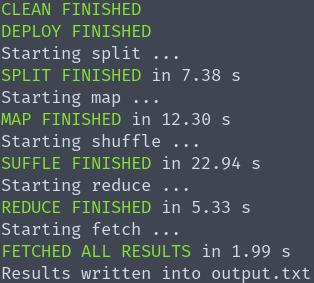
\includegraphics[width=5cm]{screenshot9.png}

On constate que cette optimisation, n'améliore malheureusement pas ou très peu la performance globale du MapReduce.

\subsection*{Gestion des pannes}
Une première amélioration consiste à vérifier le bon fonctionnement de chaque worker avant de lancer le map. Si un worker n'est pas disponible, nous découpons le fichier à mapper en un nombre incorrect de splits et nous répartirons mal nos maps. Pour éviter ce genre de problèmes, le DEPLOY a été programmé pour commenter automatiquement les workers sur lesquels le deploiement a échoué (les lignes commençant par un caraclère \# dans le fichier \texttt{machines.txt} sont ignorées). Le script MASTER appelle automatiquement le script DEPLOY en début de programme. En effectuant l'étape DEPLOY puis MASTER on s'assure que la liste de workers est à jour au moment où on lance le MASTER et que celui-ci ne tombera pas dans un cas où un de ses workers ne fonctionne pas (du moins on minimise ce risque).

Afin de détecter rapidement des anomalies, des timeout ont été rajoutées lors de l'execution des commandes mkdir en ssh. Il n'y a cependant pas de timeout sur les commandes scp (entre master et workers et entre workers seulement) pour pouvoir gérer des temps de transferts potentiellement longs.

Au moment de l'envoi des shuffles entre les workers, chaque slave effectuait au départ jusqu'à 5 tentatives en cas d'échec (configurable via une variable globale). Dans ces conditions, l'étape de shuffle échouait quasi systématiquement sur le fichier de 18.3 MB lorsque le nombre de workers excédait les 20/25. Il semblait y avoir un problème lors de l'envoi des shuffles entre workers avec scp, lorsque trop de machines tentent de se connecter simultanément à la même machine. Lors de mes tests, chaque worker parvenait à envoyer ses shuffles à toutes les autres workers lorsque le fichier SLAVE.py était executé individuellement, mais le shuffle échouait lorsque tous les scipts étaient executés en parallèle par le master.

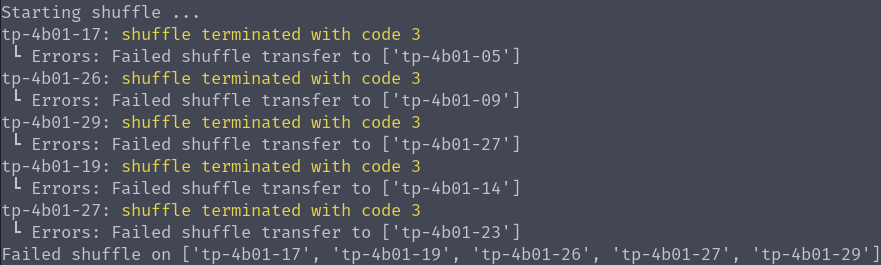
\includegraphics[width=10cm]{screenshot_shuffle7.png}

La solution a été d'augmenter le nombre maximal de tentatives d'envoi de chaque worker et de rajouter une temporisation entre chacune des tentatives. Chaque worker tente d'envoyer ses shuffles aux autres workers et en cas d'échec récupère le code d'erreur retourné par la commande scp puis attend 200 ms avant de retenter l'envoi. Il y a une distinction faite par le programme sur le code d'erreur retourné par la commande scp. Si le code d'erreur retourné est toujours 1 (c'est l'erreur qui se produit lors du phénomène observé) le programme peut faire jusqu'à 500 tentatives successives avant d'abandonner et de retourner un code d'erreur pour notifier le master. Si le code d'erreur retourné par scp n'est pas 1 (ce qui signifie que nous avons un autre type d'erreur que celui attendu), le nombre maximum de tentatives successives est de 5. Cela permet de détecter et remonter rapidement au master les anomalies qui ne sont pas dues à ces problème de surchage des workers.

Il y a un compromis à trouver sur le temps d'attente : si les tentatives ne sont pas assez espacées dans le temps, toutes les tentatives échoueront et cela génèrait beaucoup de requêtes simultanée. On ne veut cependant pas attendre trop longtemps entre chaque tentative pour ne pas trop impacter la performance globale du MapReduce. La valeur de 200ms a été trouvée de façon empirique.

On pourrait ensuite coder le master pour lancer une nouvelle tentative de shuffle sur le worker qui a échouée (relancer le script SLAVE.py sur le worker qui a échoué). On pourrait de plus en faire de même à chaque étape (map, shuffle, reduce). Ce code a été implémenté pour le shuffle comme c'est l'étape qui posait le plus de problèmes lors des tests, mais commenté pour éviter d'alourdir trop le scipt. L'idée est que si le master doit relancer une étape dans son intégralité sur un ou plusieurs workers, la performance globale du MapReduce sera lourdement impactée. Puisque le but ici est de tenter d'optimiser le code pour obtenir la meilleure performance possible, il est plus intéressant d'arrêter tout le MapReduce et de revoir le code pour optimiser l'étape qui a échouée.

\section{Vérification de la loi d'Amdahl}
La loi d'Amdahl permet de quantifier l'accéleration théorique d'un programme liée à son taux de parallélisation et le nombre de processeurs (ici le nombre de workers). Plus précisément, nous avons la formule suivante : speedup = $\frac{1}{(1-P)+(\frac{P}{N})}$ avec P le taux de parallélisation du programme et N le nombre de processeurs.

Dans notre cas le taux de parallélisation reste constant et le nombre de workers varie. Nous pouvons donc faire varier le nombre de workers et tracer la courbe de speedup empirique puis la comparer avec le speedup théorique. Puisqu'on ne connait pas la valeur de P, on prendra une valeur arbitraire qui collera avec nos observations.

Le résultat sur le fichier de 72 kB est le suivant :

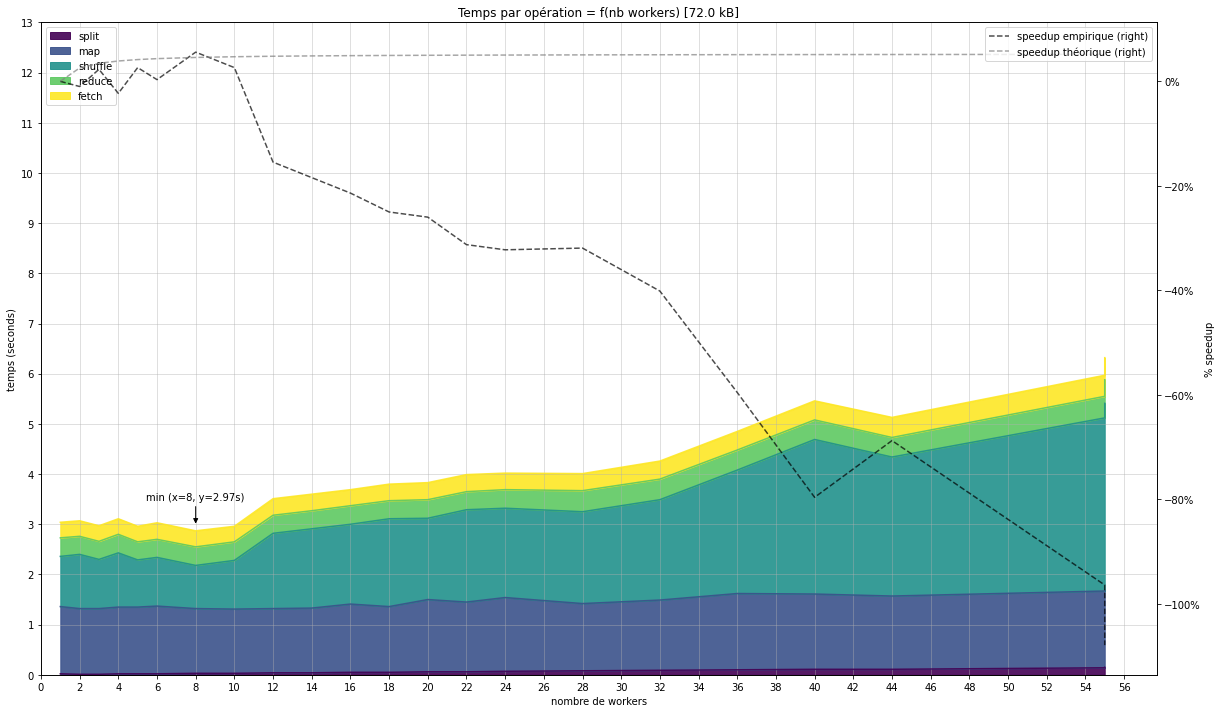
\includegraphics[width=\columnwidth]{graph0.png}

Le speedup théorique a été tracé pour P = 0.05. On peut observer ici que le MapReduce ne fait pas sens pour des fichiers de cette taille puisqu'on obtient un speedup négatif pour plus de 10/12 workers. Le meilleur temps est de 3s obtenu avec 8 workers. On obtient de plus une grande variabilité dans les résultats du fait que chaque opération prend un temps relativement court. Etudions plutôt le comportement du programme sur de plus gros fichiers.

Le résultat sur le fichier de 18.3 MB est le suivant :

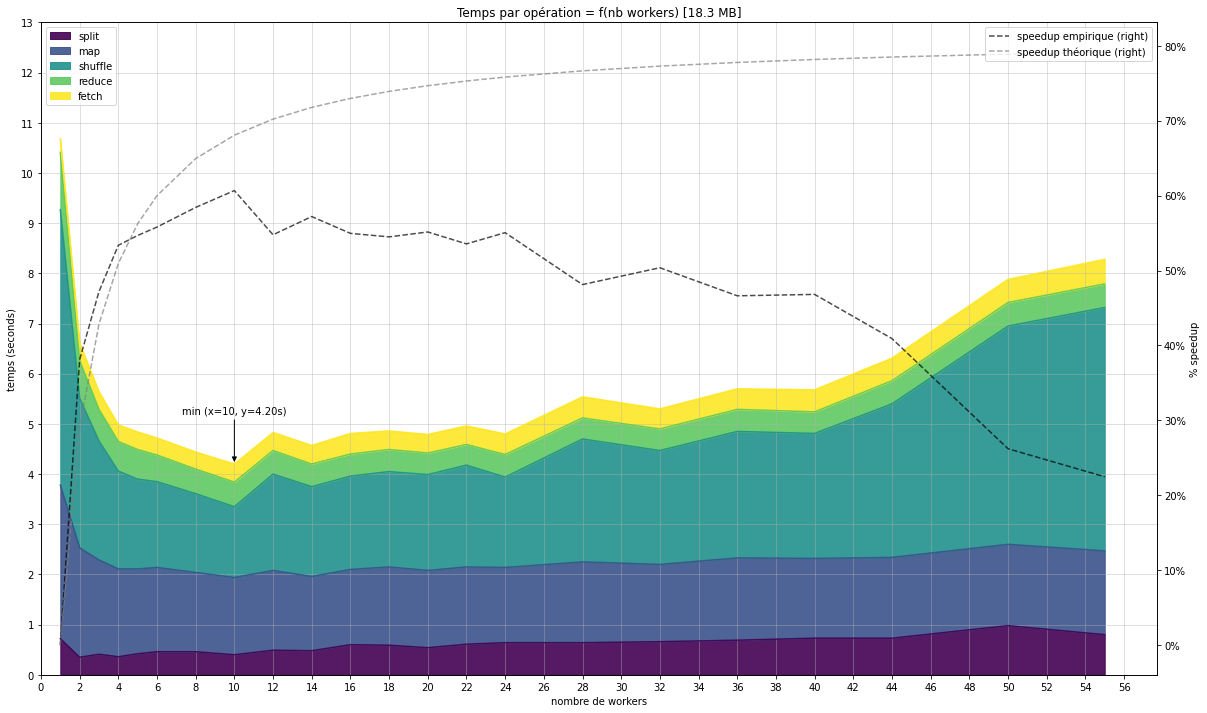
\includegraphics[width=\columnwidth]{graph1.png}

Ici, on a pris une valeur de P = 0.45. On constate que jusqu'à environ 10 workers, les courbes empiriques et théoriques sont assez proches. Au delà d'une demi-douzaine de workers, le phénomène décrit au paragraphe sur la gestion des pannes entre en jeu : chaque worker semble recevoir un nombre trop important de requêtes au moment du shuffle et doit attendre un certain temps (d'au moins 200ms) avant de pouvoir s'envoyer leurs shuffles, ce qui dégrade la performance globale du MapReduce. Il semble qu'au delà d'un certain nombre de workers, les tâches sont réparties de manières telles que chaque machine ne peut plus traiter ses tâches plus rapidement. L'ajout de workers ne fait alors qu'ajouter de la latence liée au communications entre machines sur le réseau.

Il est intéressant de constater que l'opération la plus longue pour les fichiers de 72 kB et 18.3 MB est le shuffle, suivi du map. Ces opérations consistent principalement en un scp. Il semblerait donc que les temps de transferts soient le pricinpal goulot d'étranglement ici. 

Le résultat sur le fichier de 398.8 MB est le suivant :

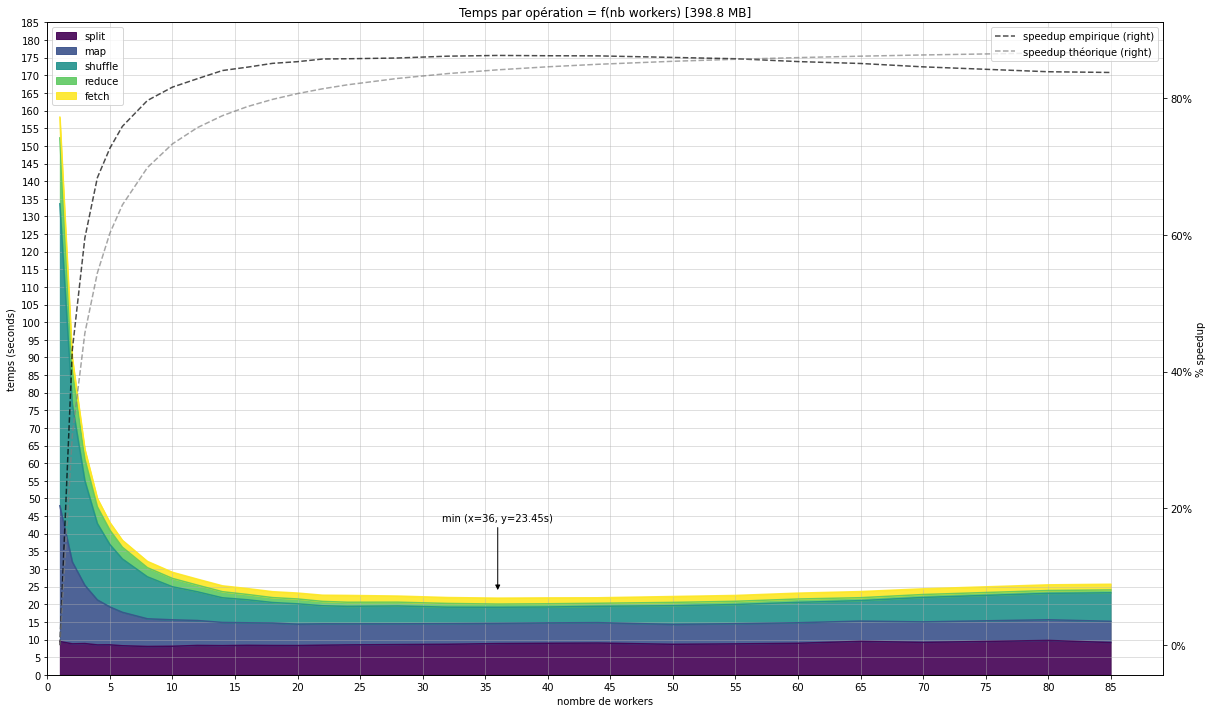
\includegraphics[width=\columnwidth]{graph2.png}

Ici la courbe de speedup empirique semble coller avec celle théorique donnée par la loi d'Amdahl avec un paramètre P = 0.47. On constate que les temps d'attente ont moins d'influence sur les résulats finaux. La tâche à réaliser pour chaque worker étant plus conséquente, on constate moins le problème de temps de traitement irréductible vu précédemment, du moins avec le nombre de workers testé.

Le résultat sur un fichier de 1.2 GB (obtenu en concaténant 3 fichiers WET) est le suivant :

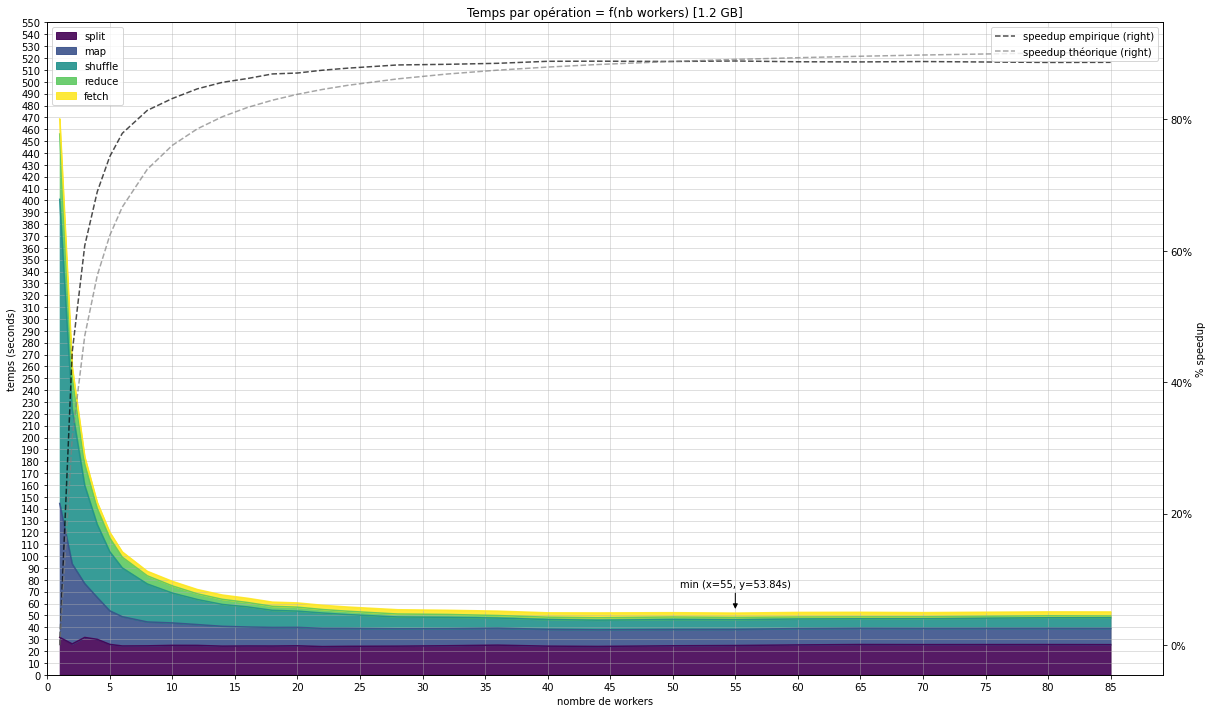
\includegraphics[width=\columnwidth]{graph3.png}

Ici la courbe de speedup empirique semble coller avec celle théorique donnée par la loi d'Amdahl avec un paramètre P = 0.48. Ici, on ne constate pas le problème de temps de traitement irréductible avec le nombre de workers testé.

Contrairement à ce que l'on a pu constater sur les deux fichiers précédents l'opération la plus longue ici est le split, suivi du shuffle et du map. Il semblerait que nous soyons ici face à une limitation liée à la puissance de calcul de nos machines. Pour améliorer encore un peu plus les performances, il serait donc intéressant d'optimiser encore plus l'étape de split.

Pour relier ces graphes entre eux on peut tracer la courbe 3D du temps total de traitement d'un fichier en fonction du nombre de workers et de la taille du fichier. Des fichiers de 191 MB et 784 MB ont été rajoutés pour avoir une meilleur vision d'ensemble :

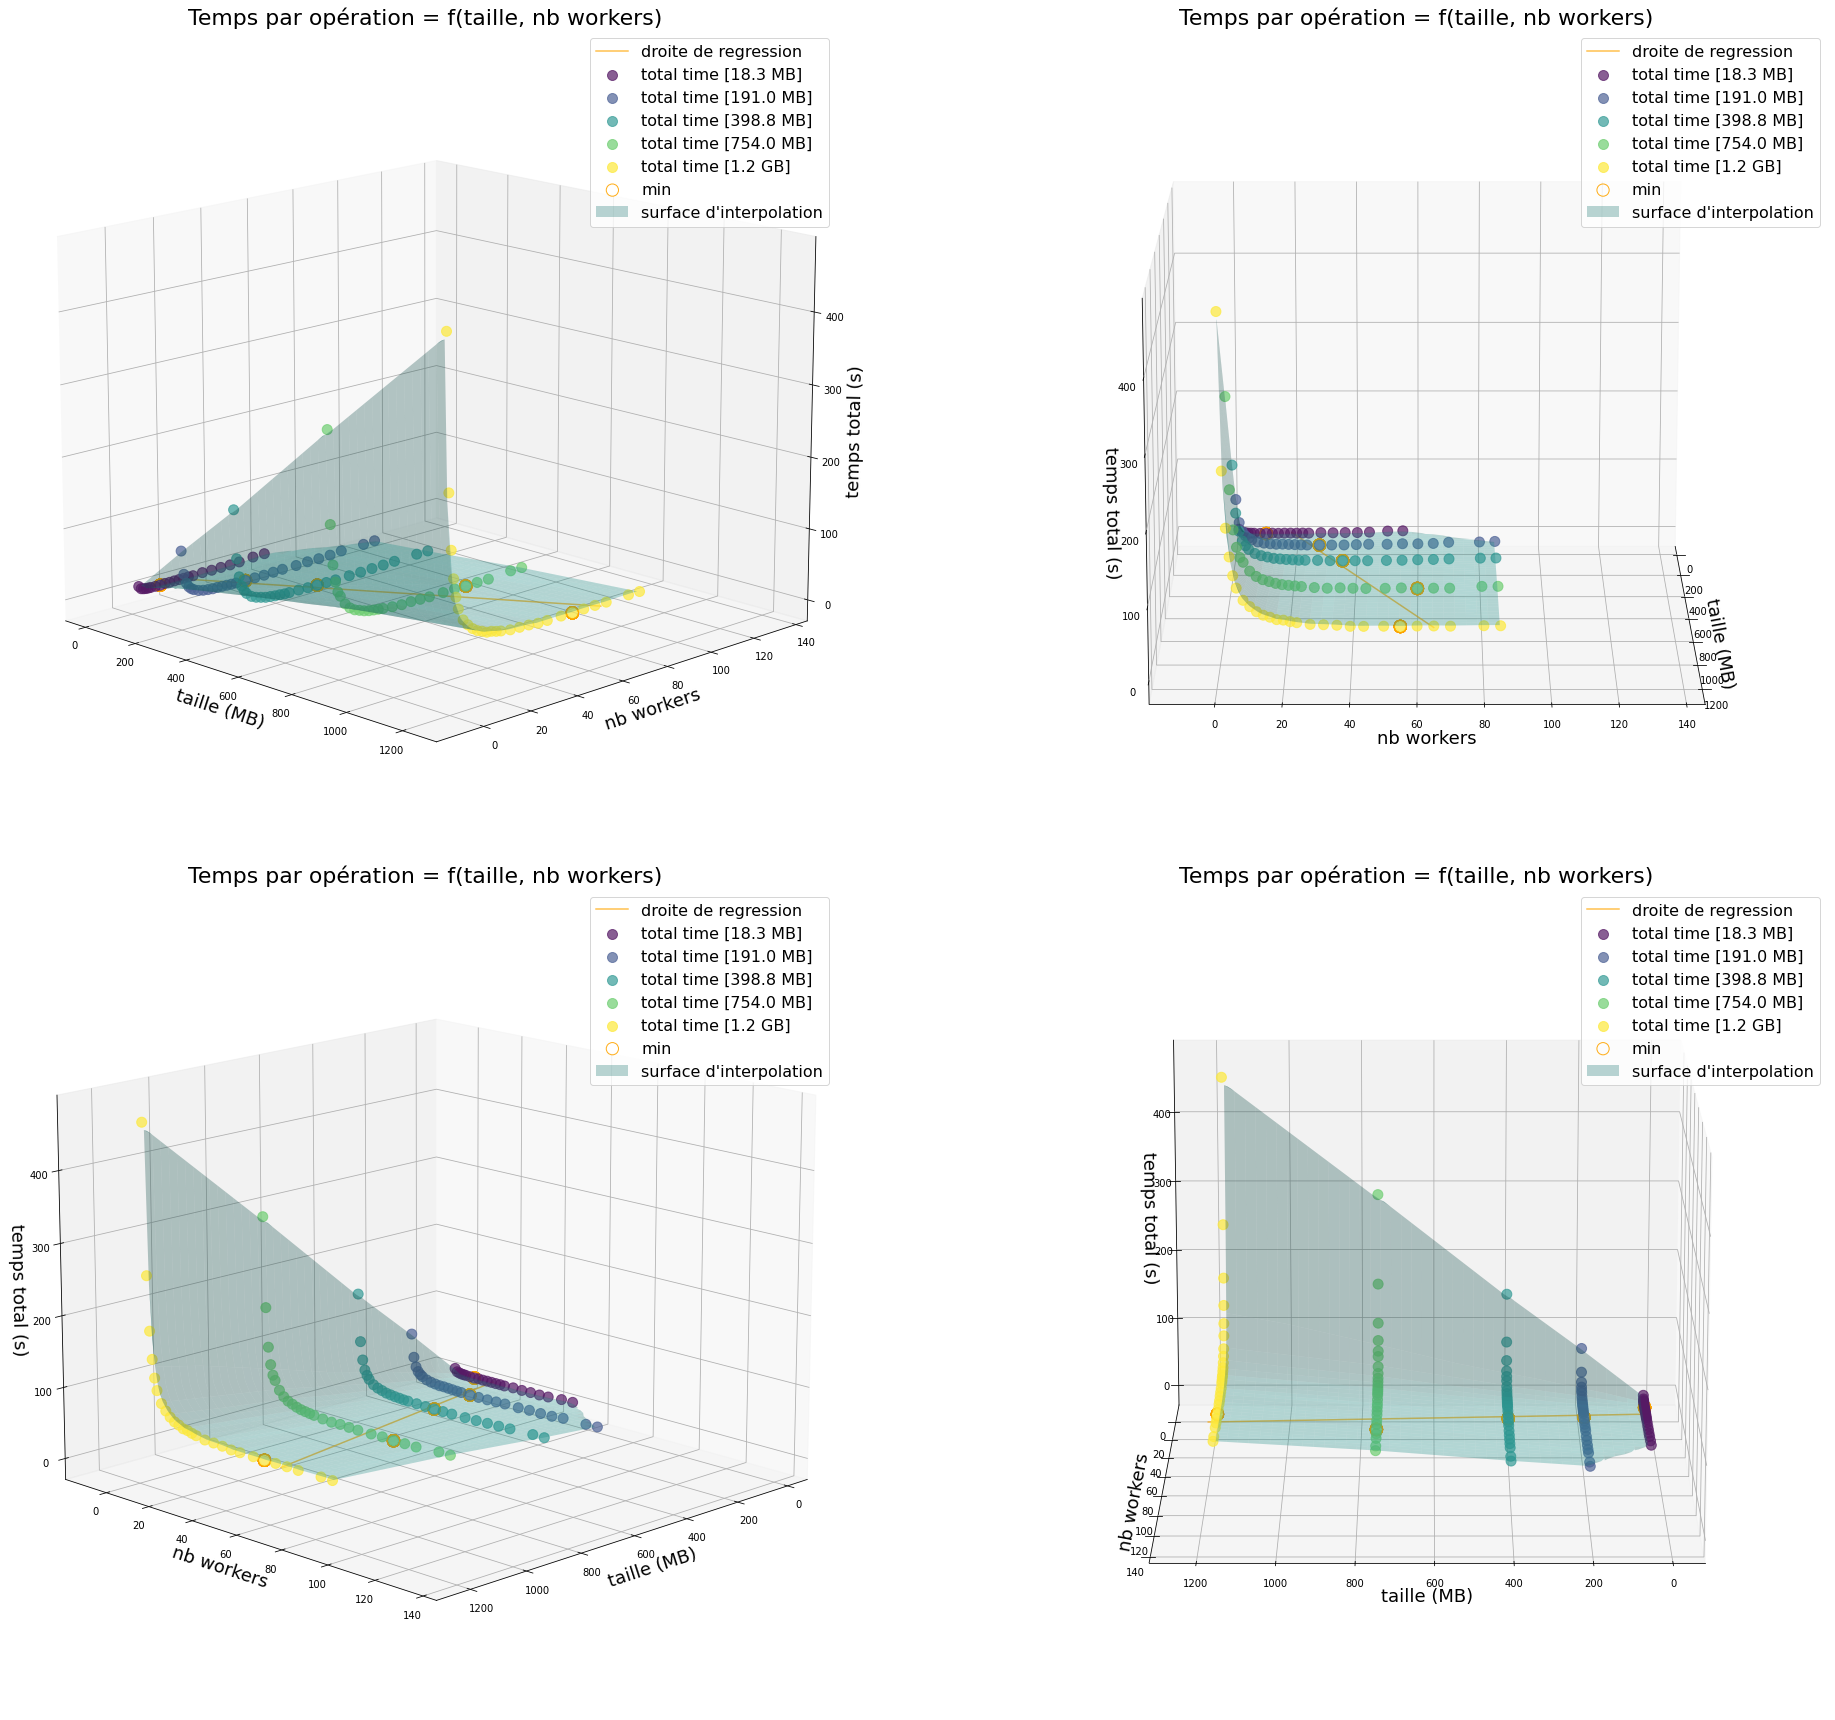
\includegraphics[width=\columnwidth]{graph4.png}

Une surface d'interpolation a été rajoutée. On constate ici que l'augmentation du la taille du fichier pour un même nombre de workers semble augmenter le temps de traitement de façon linéaire, en dehors d'une certaine limite pour de trop petits fichiers pour lesquels l'opération de MapReduce ne fait pas sens. Pour chaque taille de fichier, le meilleur temps obtenu est mis en évidence en orange, et une droite de regression a été rajoutée afin de mieux visualiser l'évolution du meilleur temps obtenu (et le nombre de workers associé) en fonction de la taille du fichier. On se rend compte qu'il y a une certaine variabilité qui rend la regression imprécise. L'idéal aurait été de pouvoir prédire avec précision le meilleur temps et le nombre de workers nécessaire en fonction de la taille du fichier.

A titre de comparaison le comptage de mots est quasi instantané sur une machine de TP en séquenciel pour le fichier de 72 kB alors que l'opération prend 2.9s sur une machine en MapReduce. On comprend alors mieux pourquoi l'opération de MapReduce ne fait pas sens dans ce cas. La quasi totalité des temps de traitements sur dûs aux opérations liées au processus de MapReduce, plutôt qu'au comptage de mots.

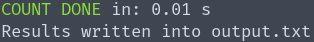
\includegraphics[width=5cm]{screenshot_seq0.png}

Le comptage prend un peu moins d'une seconde en séquenciel sur une machine de TP pour le fichier de 18.3 MB alors que notre meilleur performance en MapReduce est de 4.2s avec 10 machines.

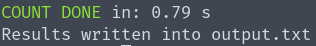
\includegraphics[width=5cm]{screenshot_seq1.png}

Sur le fichier de 398.8 MB, le MapReduce prend 28.3s en séquenciel, contre 23.6s obtenu avec 36 machines.

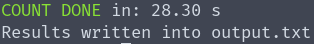
\includegraphics[width=5cm]{screenshot_seq2.png}

Enfin sur le fichier de1.2 GB, le MapReduce prend 1 min 17s, contre 53.8s obtenu avec 55 machines.

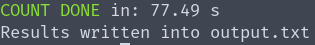
\includegraphics[width=5cm]{screenshot_seq3.png}

\section*{Conclusion}

Nous avons vu que la réalisation d'une simple tâche de comptage de mots en MapReduce nécessite la coordination et l'échange de données entre différentes machines. Cela entraine beaucoup de travaille supplémentaire et n'est justifié que dans le cas de gros volumes de données à traiter, le MapReduce ayant fait à peine mieux que le traitement en séquenciel sur les fichiers de 398.8 MB et de 1.2 GB. Il existe un certain nombre d'optimisations possibles comparé au schéma initial du MapReduce, notamment sur l'aggregation de petits fichiers et leur écriture en un seul bloc. Il faudra dans ce cas faire attention à ne pas excéder le niveau maximum de RAM des workers. Ces optimisations ont été adaptées au comptage de mot mais doivent cependant peut-être être revues pour d'autres applications.

D'après nos tests il semblerait que la loi d'Amdahl soit bien respectée, malgré des temps de latences plus importants que ceux attendus théoriquement, liés aux temps de latence réseau.

Encore une fois, les temps de latence réseau et la gestion des ressources (RAM, écritures disques) semblent être au coeur des problématiques liées à l'optimisation d'un MapReduce.

\end{document}